\documentclass[tikz]{beamer}
\usetheme[hideothersubsections]{Hannover}
\usepackage{fontspec}
\usepackage{stmaryrd,amsthm,amsmath,amssymb}
\usepackage{unicode-math}
\usepackage{color,graphicx,subfig}
\usepackage{tikz,pgfplots}
\usepackage{aircraftshapes}
\usepackage{algorithm,algpseudocode}
\usepackage{tabulary,multirow}
\usepackage{alltt}
\usepackage{booktabs}
\usepackage{pgfpages}

\setbeameroption{show notes}

\usetikzlibrary{intersections}
\usetikzlibrary{decorations.pathmorphing}

\usecolortheme{dolphin}

\DeclareMathOperator{\first}{first}

\title[Reconfiguration par Monte Carlo]{%
  Recherche arborescente Monte Carlo appliquée au problème de reconfiguration
  dynamique de l'espace aérien
}
\author[Hondet, Viry]{G.~Hondet, B.~Viry}

% ----------------------------------------------------------
% nuremotation des pages -----------------------------------
% ----------------------------------------------------------
\def\swidth{1.6cm}
\setbeamersize{sidebar width left=\swidth}
\setbeamertemplate{sidebar left}
{%
  {\usebeamerfont{title in sidebar}
    \vskip1.5em
    \usebeamercolor[fg]{title in sidebar}
    \insertshorttitle[width=\swidth,center,respectlinebreaks]\par
    \vskip1.25em
  }
  {
    \usebeamercolor[fg]{author in sidebar}
    \usebeamerfont{author in sidebar}
    \insertshortauthor[width=\swidth,center,respectlinebreaks]\par
    \vskip1.25em
  }
  \hbox to2cm{\hss\insertlogo\hss}
  \vskip1.25em
  \insertverticalnavigation{\swidth}
  \vfill
  \hbox to2cm{\hskip0.6cm\usebeamerfont{subsection in
      sidebar}\strut\usebeamercolor[fg]{subsection in
      sidebar}\insertframenumber /\inserttotalframenumber\hfill}
  \vskip3pt
}
% ----------------------------------------------------------

\begin{document}
\begin{frame}
  \titlepage{}
\end{frame}

\AtBeginSection[]
{%
  \begin{frame}
    \frametitle{Plan}
    \tableofcontents[currentsection]
  \end{frame}
}

\section*{Introduction}

\begin{frame}[c]{Introduction}
  \begin{itemize}
    \item But: diminution de la charge de travail des contrôleurs
    \item Actuellement: reconfiguration de l'espace aérien à la volée
    \item Travail expose: planification des séquences d'ouverture
    \item Comment? Algorithme stochastique de recherche arborescente
  \end{itemize}
\end{frame}
\begin{frame}[c]{Travaux actuels}
  \begin{itemize}
    \item Bloem \& Gupta, 2010, contraintes dures sur la modélisation
    \item Sergeeva \textit{et.\ al.}, 2017, coûts
    \item Gianazza, 2010, modélisation de la charge de travail
    \item Gaudel \& Sebag, 2010, Monte Carlo un joueur
  \end{itemize}
  \begin{block}{Travail présenté}
    \begin{itemize}
      \item Coût de transition en contrainte
      \item Utilisation d'une méthode stochastique
    \end{itemize}
  \end{block}
\end{frame}

\section{Modèle}
\subsection{Introduction à la charge de travail}
\begin{frame}{Introduction à la charge de travail}
  \begin{block}{Facteurs humains}
    Fatigue, stress, expérience, \dots
    \note[item]{difficulté à quantifier}
  \end{block}
  \begin{block}{Environnement}
    \begin{figure}
      \subfloat[Traffic complexe]{%
        \begin{tikzpicture}[scale=0.3]
          \node [aircraft top, fill=black, scale=4] at (2, 2) {};
          \node [aircraft top, fill=black, scale=4, rotate=30] at (3, 2) {};
          \node [aircraft top, fill=black, scale=4, rotate=230] at (4, 2) {};
          \node [aircraft top, fill=black, scale=4, rotate=180] at (4, 3) {};
          \node [aircraft top, fill=black, scale=4, rotate=300] at (5, 2) {};
          \node [aircraft top, fill=black, scale=4, rotate=110] at (3, 1) {};
          \node [aircraft top, fill=black, scale=4, rotate=147] at (2, 5) {};
          \node [aircraft top, fill=black, scale=4, rotate=24] at (1, 4) {};
          \node [aircraft top, fill=black, scale=4, rotate=54] at (7, 4) {};
          \node [aircraft top, fill=black, scale=4, rotate=93] at (7, 2) {};
          \node [aircraft top, fill=black, scale=4, rotate=211] at (3, 6) {};
          \node [aircraft top, fill=black, scale=4, rotate=200] at (3, 5) {};
          \node [aircraft top, fill=black, scale=4, rotate=100] at (4, 4) {};
          \node [aircraft top, fill=black, scale=4, rotate=350] at (2, 4) {};
          % Polygon
          \draw (3, 0) -- (8, 1) -- (8, 5) -- (4, 6) -- (1, 6) -- (0, 1) --
            cycle;
          \draw (0.2, 2) -- (3, 3);
          \draw (3, 0) -- (3, 3);
          \draw (3, 3) -- (8, 3);
          \draw (6, 5.5) -- (6, 3);
          \draw (3, 3) -- (4, 6);
        \end{tikzpicture}
      }\qquad
      \subfloat[Traffic simple]{%
        \begin{tikzpicture}[scale=0.3]
          \node [aircraft top, fill=black, scale=4, rotate=45] at (2, 1) {};
          \node [aircraft top, fill=black, scale=4] at (4, 2) {};
          \node [aircraft top, fill=black, scale=4] at (5, 2) {};
          \node [aircraft top, fill=black, scale=4] at (7, 2) {};
          \node [aircraft top, fill=black, scale=4,rotate=270] at (2, 5) {};
          \node [aircraft top, fill=black, scale=4,rotate=270] at (2, 3) {};

          % Polygon
          \draw (3, 0) -- (8, 1) -- (8, 5) -- (4, 6) -- (1, 6) -- (0, 1) --
            cycle;
          \draw (0.2, 2) -- (3, 3);
          \draw (3, 0) -- (3, 3);
          \draw (3, 3) -- (8, 3);
          \draw (6, 5.5) -- (6, 3);
          \draw (3, 3) -- (4, 6);
        \end{tikzpicture}
      }
    \end{figure}
    \note[item]{Expliquer complexité sur image}
  \end{block}
\end{frame}


\subsection{Espace aérien}
\begin{frame}{Fragmentation de l'espace}
  \begin{figure}
    \centering
    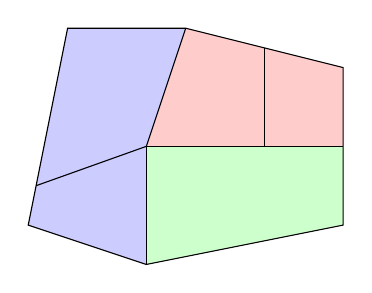
\begin{tikzpicture}[scale=0.5]
      \fill [red!20] (3, 3) -- (8, 3) -- (8, 5) -- (4, 6) -- cycle;
      \fill [green!20] (3, 0) -- (8, 1) -- (8, 3) -- (3, 3) -- cycle;
      \fill [blue!20] (0, 1) -- (3, 0) -- (3, 3) -- (4, 6) -- (1, 6) -- cycle;

      % Polygon
      \draw (3, 0) -- (8, 1) -- (8, 5) -- (4, 6) -- (1, 6) -- (0, 1) -- cycle;
      \draw (0.2, 2) -- (3, 3);
      \draw (3, 0) -- (3, 3);
      \draw (3, 3) -- (8, 3);
      \draw (6, 5.5) -- (6, 3);
      \draw (3, 3) -- (4, 6);
    \end{tikzpicture}
    \caption{Découpage de l'espace aérien}
  \end{figure}
  \note[item]{Module elementaire}
  \note[item]{Secteur \(=\) work position}
  \note[item]{Partition}
\end{frame}
\begin{frame}{Contexte}
  \begin{block}{Justification}
    Seuls certains secteurs sont pertinents
    \note[item]{Pour alléger la workload, éviter e.g.\ la non convexité}
  \end{block}
  \begin{figure}
    \subfloat[Secteur invalide] {%
      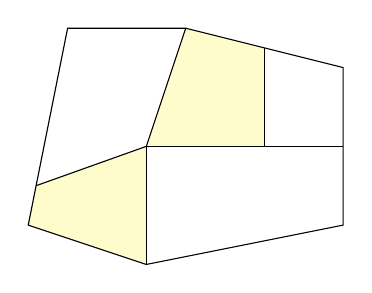
\begin{tikzpicture}[scale=0.5]
        \fill [yellow!20] (0, 1) -- (0.2, 2) -- (3, 3) -- (3, 0) -- cycle;
        \fill [yellow!20] (3, 3) -- (6, 3) -- (6, 5.5) -- (4, 6) -- cycle;

        % Polygon
        \draw (3, 0) -- (8, 1) -- (8, 5) -- (4, 6) -- (1, 6) -- (0, 1) -- cycle;
        \draw (0.2, 2) -- (3, 3);
        \draw (3, 0) -- (3, 3);
        \draw (3, 3) -- (8, 3);
        \draw (6, 5.5) -- (6, 3);
        \draw (3, 3) -- (4, 6);
      \end{tikzpicture}
    } \quad \pause{}
    \subfloat[Secteur valide] {%
      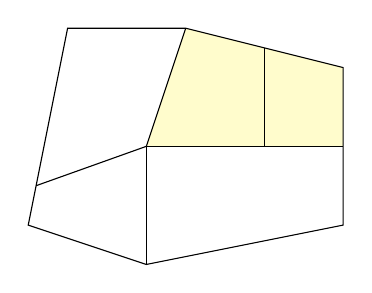
\begin{tikzpicture}[scale=0.5]
        \fill [yellow!20] (3, 3) -- (8, 3) -- (8, 5) -- (4, 6) -- cycle;

        % Polygon
        \draw (3, 0) -- (8, 1) -- (8, 5) -- (4, 6) -- (1, 6) -- (0, 1) -- cycle;
        \draw (0.2, 2) -- (3, 3);
        \draw (3, 0) -- (3, 3);
        \draw (3, 3) -- (8, 3);
        \draw (6, 5.5) -- (6, 3);
        \draw (3, 3) -- (4, 6);
      \end{tikzpicture}
    }
  \end{figure}
  \pause{}
  \begin{block}{Contexte}
    Restreint l'ensemble de secteurs utilisables
  \end{block}
\end{frame}
\begin{frame}{Transitions}
  \begin{block}{Notion de temps}
    Sequencage d'une journée par pas de temps réguliers
  \end{block}
  \begin{block}{Transition}
    \begin{itemize}
      \item Une reconfiguration éventuelle par pas de temps
      \item Trois types de reconfiguration: \emph{fusion}, \emph{séparation} ou
        \emph{transfert}
    \end{itemize}
  \end{block}
  \begin{block}{Contraintes}
    Pas de reconfiguration trop lourde
  \end{block}
\end{frame}
\begin{frame}[c]{Transitions}
  \begin{block}{Fusion, séparation}
    \begin{figure}
      \subfloat[Fusionné]{%
        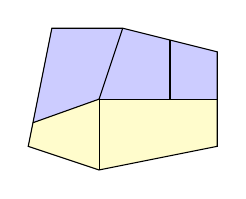
\begin{tikzpicture}[scale=0.3]
          \fill [yellow!20] (3, 0) -- (8, 1) -- (8, 3) -- (3, 3) -- (0.2, 2) --
            (0, 1) -- cycle;
          \fill [blue!20] (0.2, 2) -- (3, 3) -- (8, 3) -- (8, 5) -- (4, 6) --
            (1, 6) -- cycle;

          % Polygon
          \draw (3, 0) -- (8, 1) -- (8, 5) -- (4, 6) -- (1, 6) -- (0, 1) --
            cycle;
          \draw (0.2, 2) -- (3, 3);
          \draw (3, 0) -- (3, 3);
          \draw (3, 3) -- (8, 3);
          \draw (6, 5.5) -- (6, 3);
          \draw (3, 3) -- (4, 6);
        \end{tikzpicture}
      }\quad \(\leftrightarrow\) \quad
      \subfloat[Séparé]{%
        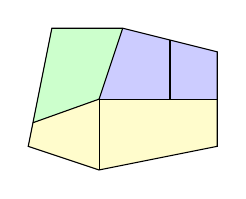
\begin{tikzpicture}[scale=0.3]
          \fill [yellow!20] (3, 0) -- (8, 1) -- (8, 3) -- (3, 3) -- (0.2, 2) --
            (0, 1) -- cycle;
          \fill [blue!20] (3, 3) -- (8, 3) -- (8, 5) -- (4, 6) -- cycle;
          \fill [green!20] (0.2, 2) -- (3, 3) -- (4, 6) -- (1, 6) -- cycle;

          % Polygon
          \draw (3, 0) -- (8, 1) -- (8, 5) -- (4, 6) -- (1, 6) -- (0, 1) --
            cycle;
          \draw (0.2, 2) -- (3, 3);
          \draw (3, 0) -- (3, 3);
          \draw (3, 3) -- (8, 3);
          \draw (6, 5.5) -- (6, 3);
          \draw (3, 3) -- (4, 6);
        \end{tikzpicture}
      }
    \end{figure}
  \end{block}
  \pause{}
  \begin{block}{Transfert}
    \begin{figure}
      \subfloat[Avant transfert]{%
        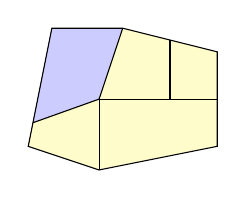
\begin{tikzpicture}[scale=0.3]
          \fill [yellow!20] (3, 0) -- (8, 1) -- (8, 5) -- (4, 6) -- (3, 3) --
            (0.2, 2) -- (0, 1) -- cycle;
          \fill [blue!20] (0.2, 2) -- (3, 3) -- (4, 6) -- (1, 6) -- cycle;

          % Polygon
          \draw (3, 0) -- (8, 1) -- (8, 5) -- (4, 6) -- (1, 6) -- (0, 1) -- cycle;
          \draw (0.2, 2) -- (3, 3);
          \draw (3, 0) -- (3, 3);
          \draw (3, 3) -- (8, 3);
          \draw (6, 5.5) -- (6, 3);
          \draw (3, 3) -- (4, 6);
        \end{tikzpicture}
      }\quad\phantom{\(\leftrightarrow\)}\quad
      \subfloat[Après transfert]{%
        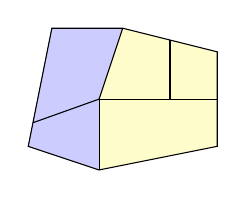
\begin{tikzpicture}[scale=0.3]
          \fill [yellow!20] (3, 0) -- (8, 1) -- (8, 5) -- (4, 6) -- (3, 3) --
            cycle;
          \fill [blue!20] (0.2, 2) -- (0, 1) -- (3, 0) -- (3, 3) -- (4, 6) --
            (1, 6) -- cycle;

          % Polygon
          \draw (3, 0) -- (8, 1) -- (8, 5) -- (4, 6) -- (1, 6) -- (0, 1) -- cycle;
          \draw (0.2, 2) -- (3, 3);
          \draw (3, 0) -- (3, 3);
          \draw (3, 3) -- (8, 3);
          \draw (6, 5.5) -- (6, 3);
          \draw (3, 3) -- (4, 6);
        \end{tikzpicture}
      }
    \end{figure}
  \end{block}
\end{frame}

\subsection{Modélisation de la charge de travail}
\begin{frame}{Modélisation de la charge de travail}
  \begin{block}{Classes}
    Trois classes de charge de travail:
    \begin{itemize}
      \item underload,
      \item overload,
      \item normal load.
    \end{itemize}
  \end{block}
  \begin{block}{Modèle de classification d'un secteur}
    Dépend du nombre d'avions
    \begin{figure}
      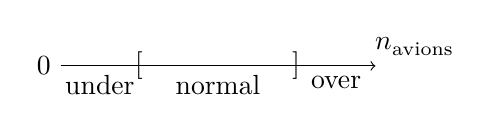
\begin{tikzpicture}
        \draw[->] (0, 0) -- (4, 0);

        \draw (0, 0) node[left] {0};
        \draw (4.5, 0) node[above] {\(n_\text{avions}\)};
        \draw (1, 0) node {\([\)};
        \draw (3, 0) node {\(]\)};
        \draw (0.5, 0) node[below] {under};
        \draw (2, 0) node[below] {normal};
        \draw (3.5, 0) node[below] {over};
      \end{tikzpicture}
    \end{figure}
  \end{block}
\end{frame}


\subsection{Construction de la fonction objectif}
\begin{frame}{Cout de partition}
  \begin{block}{Agglomération des classifications}
    \note[item]{Passage des secteurs a la partition}
    Trois coûts intermédiaires
    \begin{itemize}
      \item sous charge \(c_-\),
      \item sur charge \(c_+\),
      \item charge normal \(c_=\).
    \end{itemize}
  \end{block}
  \begin{block}{Coût résultant}
    Coût d'une partition \(P\) à un temps \(t\):
    \begin{equation}
      C(P,t) = \alpha c_+ + \beta c_= + \gamma c_- + \lambda \vert P \vert
    \end{equation}
    \note[item]{Expliquer provenance de \(|P|\)}
    \note[item]{Utilisation typique des coefficients}
  \end{block}
\end{frame}
\begin{frame}[c]{Coût de transition}
  \begin{block}{Signification}
  Coordination entre contrôleurs
  \end{block}
  \begin{equation}
    C_\text{tr}(P_1, P_2) =
    \begin{cases}
      0 & \text{si\;} P_1 = P_2\\
      \theta & \text{sinon}
    \end{cases}
  \end{equation}
\end{frame}
\begin{frame}[c]{Fonction objectif}
  Coût d'une séquence de partitions \(\pi = [P_0, \dots, P_n]\),
  \begin{equation}
    f(\pi) = C(P_0, t_0) + \sum_{i=1}^n \left[
      C(P_i, t_i) + C_\text{tr}(P_{i-1}, P_i)
    \right]
  \end{equation}
\end{frame}

\section{Méthode de résolution}
\subsection{Principe}
\begin{frame}[c]{Principe}
  \begin{block}{Recherche arborescente de Monte Carlo}
    \begin{itemize}
      \item Parcours meilleur en premier
      \item Recherche stochastique
      \item Recherche d'un chemin par maximisation
      \item Évaluation des chemins par simulations de Monte Carlo
    \end{itemize}
  \end{block}
  \begin{block}{Arbres}
    \begin{itemize}
      \item Arbre de recherche
      \item Arbre de modèle
    \end{itemize}
  \end{block}
\end{frame}

\subsection{Utilisation du modèle}
\begin{frame}[c]{Utilisation du modèle}
  \begin{block}{Production (arbre de modèle)}
    \begin{figure}
    \begin{center}
      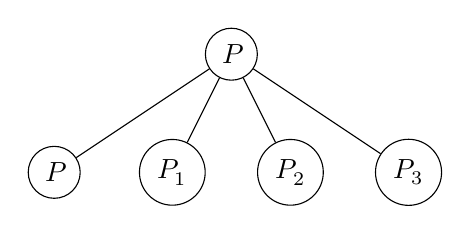
\begin{tikzpicture}[scale=1]
      \node [circle, draw] {\(P\)}
        child {node [circle, draw] {\(P\)}}
        child {node [circle, draw] {\(P_1\)}}
        child {node [circle, draw] {\(P_2\)}}
        child {node [circle, draw] {\(P_3\)}};
    \end{tikzpicture}
    \end{center}
    \caption{Représentation des transitions, \(P_1, P_2\) et \(P_3\)
    atteignables depuis \(P\)}
    \end{figure}
  \end{block}
  \begin{block}{N\oe{}ud (arbre de recherche)}
    \begin{itemize}
      \item Partition
      \item Espérance de gain
    \end{itemize}
    \note{Espérance de gain \(\sim 1/f\)}
  \end{block}
\end{frame}

\subsection{Phases}
\begin{frame}[t]{Sélection et expansion}
  \begin{columns}
    \begin{column}{0.5\textwidth}
      \begin{block}{Sélection}
        Choix d'un chemin par méthode de bandits
        \note[item]{choix des nœuds prometteurs \(\rightarrow\) exploitation v.\
        exploration \(\rightarrow\) \emph{bandit} methods}
        \begin{figure}
          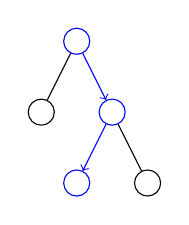
\begin{tikzpicture}[scale=0.6]
            \node [circle, draw, blue] {}
              child {node [circle, draw] {}}
              child[->, blue] {%
                node [circle, draw] {}
                child {node [circle, draw] {}}
                child[-, black] {node [circle, draw] {}}
              };
          \end{tikzpicture}
          \caption{Sélection d'un chemin}
        \end{figure}
      \end{block}
    \end{column}
    \pause{}
    \begin{column}{0.5\textwidth}
      \begin{block}{Expansion}
        Ajout d'un n\oe{}ud
        \begin{figure}
          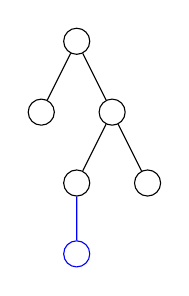
\begin{tikzpicture}[scale=0.6]
            \node [circle, draw] {}
              child {node [circle, draw] {}}
              child {%
                node [circle, draw] {}
                child {%
                  node [circle, draw] {}
                  child [circle, draw, blue] {node [circle, draw] {}}
                }
                child {node [circle, draw] {}}
              };
          \end{tikzpicture}
          \caption{Expansion}
        \end{figure}
      \end{block}
    \end{column}
  \end{columns}
\end{frame}
\begin{frame}[t]{Simulation et sauvegarde}
  \begin{columns}
    \begin{column}{0.5\textwidth}
      \begin{block}{Simulation}
        Choix d'un chemin aléatoire partant du n\oe{}ud jusqu'à une feuille
        \note[item]{Évaluer le cout d'un chemin passant par le nœud ajouté}
        \begin{figure}
          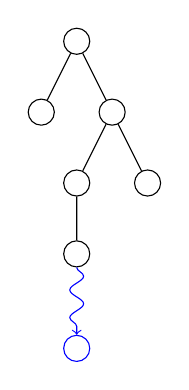
\begin{tikzpicture}[scale=0.6]
            \node [circle, draw] {}
              child {node [circle, draw] {}}
              child {%
                node [circle, draw] {}
                child {%
                  node [circle, draw] {}
                  child [circle, draw] {node (l) [circle, draw] {}}
                }
                child {node [circle, draw] {}}
              };

            \draw[blue] (l) ++(0, -2) node(s) [circle, draw] {};
            \draw[->, blue, decorate, decoration={snake}] (l) -- (s);
          \end{tikzpicture}
        \caption{Simulation}
        \end{figure}
      \end{block}
    \end{column}
    \pause{}
    \begin{column}{0.5\textwidth}
      \begin{block}{Sauvegarde}
        Mise à jour de l'arbre de recherche
        \note[item]{Complète les statistiques}
      \end{block}
      \begin{figure}
        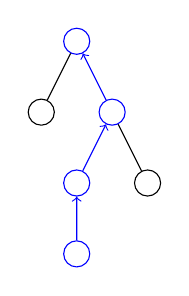
\begin{tikzpicture}[scale=0.6]
          \node [circle, draw, blue] {}
            child {node [circle, draw] {}}
            child[<-, blue] {%
              node [circle, draw] {}
              child {%
                node [circle, draw] {}
                child [circle, draw] {node [circle, draw] {}}
              }
              child[-, black] {node [circle, draw] {}}
            };
        \end{tikzpicture}
        \caption{Sauvegarde}
      \end{figure}
    \end{column}
  \end{columns}
\end{frame}
\begin{frame}[c]{Algorithme MCTS}
  \note[item]{Critère d'arrêt: temps ou mémoire}
  \begin{algorithmic}
    \Procedure{MctsSearchTree}{$u$}
    \While{critère d'arrêt non atteint}
      \State{}\(\pi \gets\)\Call{Sélection}{$u$}
      \State{}\(v \gets\)\Call{Expansion}{$\pi$}
      \State{}\(\Delta \gets\)\Call{Simulation}{$v$}
      \State{}\Call{Sauvegarde}{$\pi$, $\Delta$}
    \EndWhile{}
    \EndProcedure{}
  \end{algorithmic}
  \note[item]{Opère en place sur l'arbre}
\end{frame}
\subsection{Construction de la solution}
\begin{frame}[c]{Construction de la solution, 1}
  \note[item]{Un appel de MctsSearchTree donne un nœud, à la jeux: un mcts pour
  un coup joué}
  \note[item]{Choix nouvelle racine
    \(\mathup{argmax}\{\mu_v | v \text{\,enfants de\,} u\}\)}
  \begin{figure}
    \begin{tikzpicture}
      \node [circle, draw, red] {}
        child[blue] {node [circle, draw] {}}
        child[blue] {node [circle, draw] {}}
        child[blue] {node [circle, draw] {}
          child {node [circle, draw] {}}
          child {node [circle, draw] {}}
          child {node [circle, draw] {}}
        }
      \end{tikzpicture}
      \caption{Première itération}
    \end{figure}
\end{frame}
\begin{frame}[c]{Construction de la solution, 2}
  \begin{figure}
    \begin{tikzpicture}
      \node [circle, draw, red] {}
        child[gray] {node [circle, draw] {}}
        child[gray] {node [circle, draw] {}}
        child {node [circle, draw, red] {}
          child[blue] {node [circle, draw] {}}
          child[blue] {node [circle, draw] {}}
          child[blue] {node [circle, draw] {}}
        }
      \end{tikzpicture}
      \caption{Deuxième itération}
    \end{figure}
\end{frame}

\subsection{A\(^*\) et glouton}
\begin{frame}[c]{A\(^*\) et glouton}
  \begin{block}{Glouton}
    Nœud de cout le plus faible sélectionné.
  \end{block}
  \begin{block}{A\(^*\) principe}
    \begin{itemize}
      \item Méthode exacte
      \item Meilleur en premier
      \item Utilisation d'une heuristique
    \end{itemize}
  \end{block}
  \begin{block}{Heuristique}
    \begin{itemize}
      \item utilisation des partitions optimales, même si non atteignables
      \item \(h(u) = \sum_{i=k+1}^f C(P^*_i, t_i)\)
        \note{%
          \(h(u)\): estimation du coût du chemin allant de \(u\)
          jusqu'à une feuille
        }
    \end{itemize}
  \end{block}
\end{frame}

\section{Résultats}
\subsection{Résultats qualitatifs}
\begin{frame}[c]{Profil}
  \note[item]{Présenter le scénario}
    \begin{figure}
      \begin{tikzpicture}
        \begin{axis}
          [line width=0.05, mark size=0.1, xlabel=pas de temps,
          ylabel=nbre de secteurs,
          legend entries={A\(^*\), MCTS}]
          \foreach \i in {0,1}{%
            \addplot+ table [
              x expr={\lineno}, y index=\i
              ]
              {./data/grouping.data};
          }
        \end{axis}
      \end{tikzpicture}
    \end{figure}
\end{frame}
\begin{frame}[c]{Comportement détaillé MCTS}
  \begin{scriptsize}
    \begin{alltt}
      \begin{tabular}{lr}
        (1 5, d) (2 3, a) (4, s4) & \multirow{5}{20mm}{\textsf{Tout surchargé}}\\
        (3, s3) (2, s2) (1 5, d) (4, s4) & \\
        (5, s5) (1, s1) (3, s3) (2, s2) (4, s4) & \\
        (5, s5) (1, s1) (3, s3) (2, s2) (4, s4) & \\
        (5, s5) (1, s1) (3, s3) (2, s2) (4, s4) & \\
        \midrule
        (1 2, g) (5, s5) (3, s3) (4, s4) & \multirow{6}{20mm}{\textsf{Tout sous
        chargé}}\\
        (4 5, c) (1 2, g) (3, s3) & \\
        (1 2 3, e) (4 5, c) & \\
        (1 2 3 4 5, f) & \\
        (1 2 3 4 5, f) & \\
        (4 5, c) (1 2 3, e) & \\
        \midrule
        (5, s5) (4, s4) (1 2 3, e) & \multirow{3}{20mm}{\textsf{5 et 4
        chargés, 1, 2 et 3 sous chargés}}\\
        (5, s5) (4, s4) (1 2 3, e) & \\
        (5, s5) (4, s4) (1 2 3, e) & \\
      \end{tabular}
    \end{alltt}
  \end{scriptsize}
\end{frame}

\subsection{Résultats quantitatifs}
\begin{frame}[c]{Résultats quantitatifs}
\begin{table}
  \centering
  \begin{tabulary}
    {\textwidth}{LRR}
    Alg.    & Cost  & Err.   \\
    \toprule
    A\(^*\) & 77.31 & 0\%    \\
    MCTS    & 82.48 & 6.7\%  \\
    Greedy  & 90.50 & 17.1\% \\
  \end{tabulary}
  \caption{Comparaison des différentes méthodes}\label{tab:methods_compare}
\end{table}
\note{Introduire les limitations}
\end{frame}
\section*{Conclusion}
\begin{frame}[c]{Conclusion}
  \begin{block}{Résultats}
    Résultats encourageants mais pas vraiment concrets
  \end{block}
  \begin{block}{Perspectives}
    Beaucoup de tests à faire,
    \begin{itemize}
      \item plus de trafic,
      \item plus gros centres,
      \item vrai trafic,
      \item modèle de charge de travail plus fin.
    \end{itemize}
  \end{block}
\end{frame}
\end{document}
